\documentclass[11pt]{article}
\usepackage{graphicx}
\usepackage[a4paper, margin=1in]{geometry}
\usepackage{times} % Use Times font
\usepackage{authblk} % Package for superscript affiliations
\usepackage{graphicx} % Package for handling citations

\begin{document}

% Header with logo
\begin{minipage}{0.2\textwidth}
    
\includegraphics[width=\textwidth]{Logo_header.pdf}
\end{minipage}
\hfill
\begin{minipage}{0.75\textwidth}
   % \centering
    \fontsize{8}{10}\selectfont % Set font size to 8
    \textbf{Joint event Euromech Colloquium on Data-Driven Fluid Dynamics/2nd ERCOFTAC Workshop on Machine Learning for Fluid Dynamics, 2-4 April 2025, London, UK}
\end{minipage}

% Abstract section
\begin{center}
  { \fontsize{16}{10} \textbf{Abstract Title Here} } \\
    \vspace{0.5cm}
    \normalsize \textbf{Author Name(s)$^{1,2}$} \\ % Example of superscript for affiliations
  { \fontsize{9}{10}\selectfont  \textit{$^1$ Affiliation 1, $^2$ Affiliation 2} } \\ % Example of superscript for multiple affiliations
  { \fontsize{9}{10}\textit{Corresponding author: Author Name (email@example.com)}} \\
\end{center}

\noindent
% Abstract content
Your abstract text goes here.  { \bf The maximum limit is 1 page.} This is a placeholder for the abstract content, which should provide a concise summary of the main points of your research, including the background, methods, results, and conclusions.  This is a sample abstract where we cite a reference \cite{sample1}.

\vspace{1cm} % Adjust space after header
\begin{figure}[htbp]
    \centering
    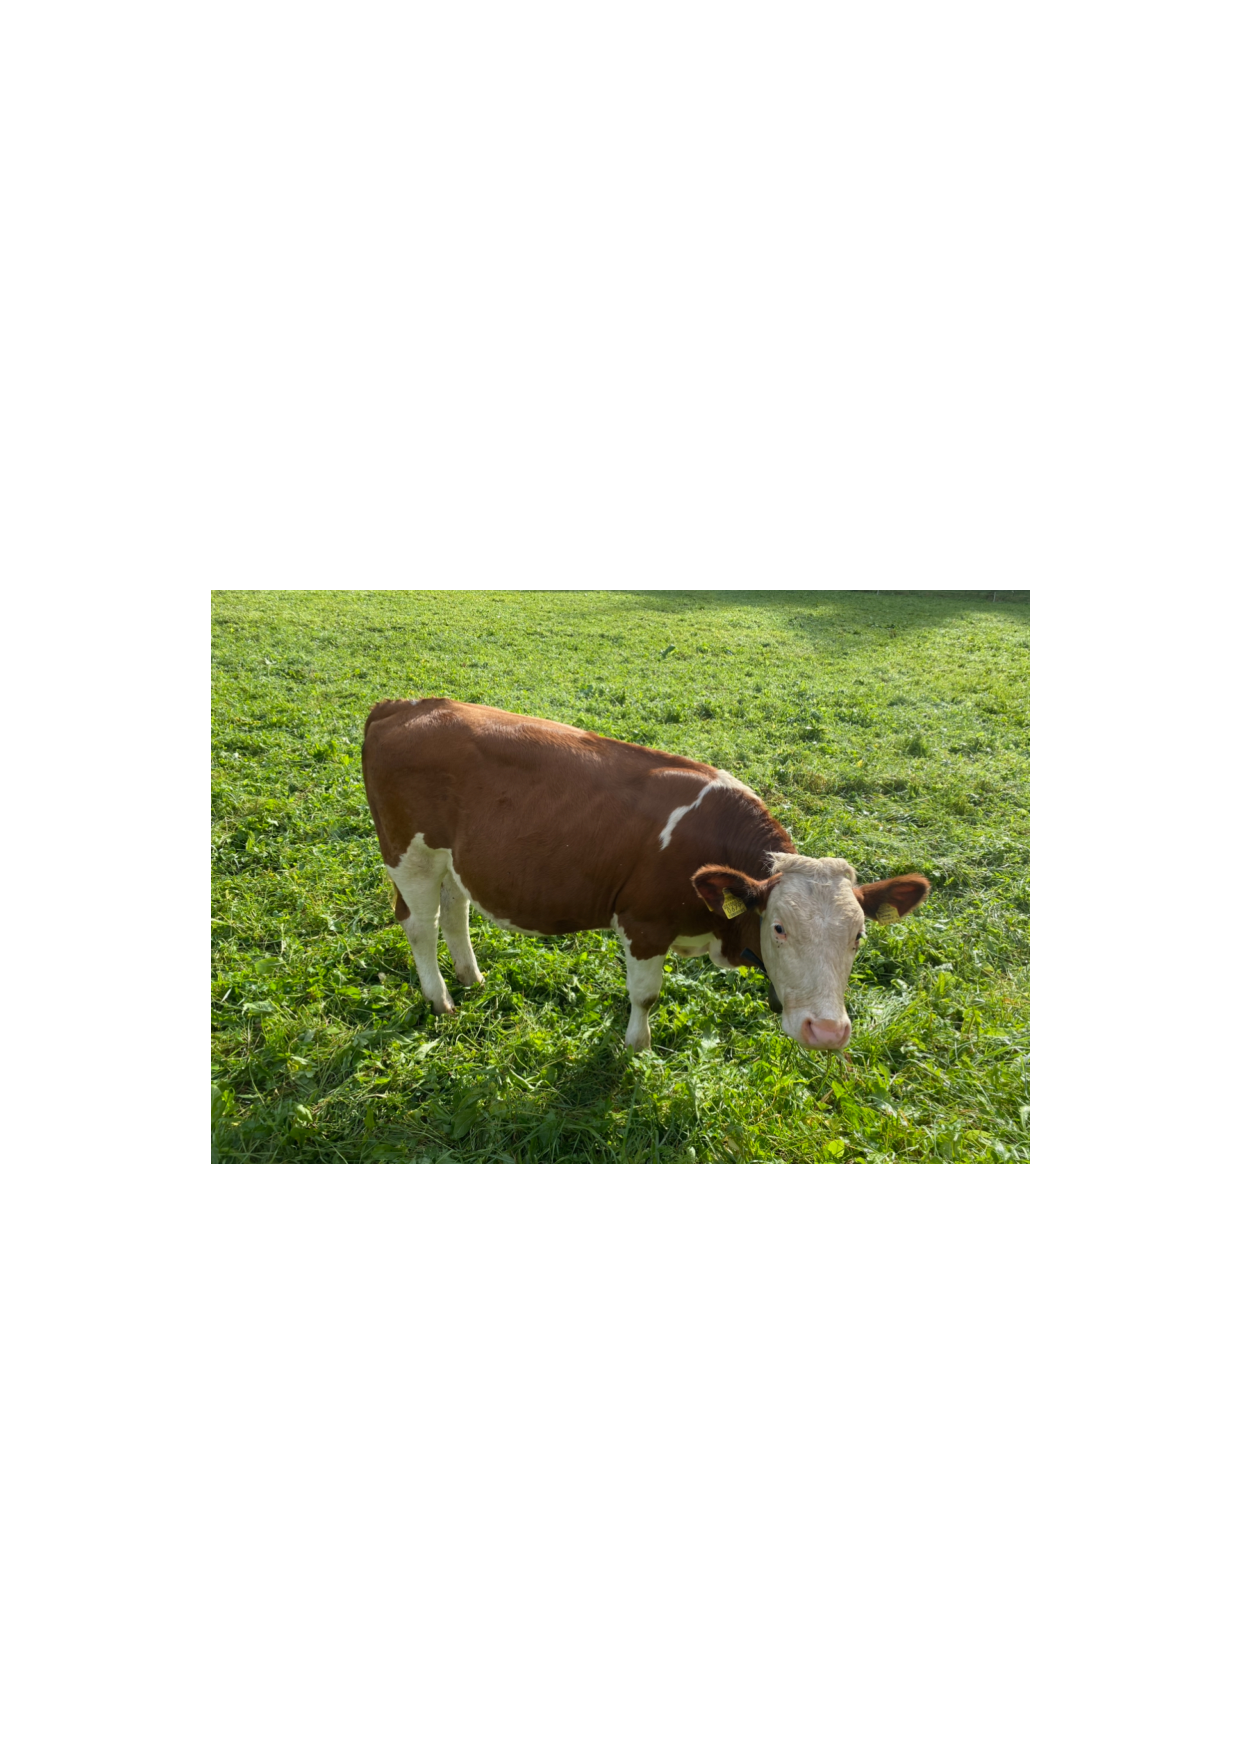
\includegraphics[width=0.7\textwidth]{sample_figure.pdf}
    \caption{Sample figure caption.}
    \label{fig:sample}
\end{figure}

\bibliographystyle{unsrt}
\bibliography{references.bib}

 
\end{document}


